\subsection{Приведенное количество теплоты. Равенство Клаузиуса. Энтропия. Энтропия идеального газа.}

\textbf{Энтропия} - это функция её состояния,

\subsubsection*{Равенство Клаузиуса. II принцип термодинамики для обратимых процессов}
\begin{figure}[H]
	\centering
	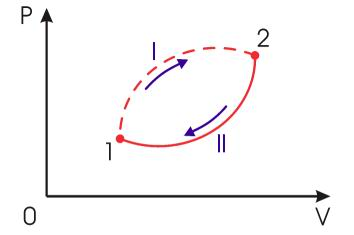
\includegraphics[width=0.7\linewidth]{image/Rule}
	\caption{График $pV$-диаграммы.
		Кривые I и II представляют разные термодинамические процессы между состояниями 1 и 2.}
	\label{fig:9}
\end{figure}
Из его равенства вытекает важное следствие. Приведенное количество теплоты при конечном обратимом переходе не зависит от пути, а зависит от:
\begin{align} \label{34.1}
	\boxed{\oint \frac{dQ}{T} = 0}
\end{align}
\begin{align} \label{34.2}
	\int\limits_{1\,I\,2} \frac{dQ}{T} + \int\limits_{2\,II\,1} \frac{dQ}{T} = 0
\end{align}

Математическая формула II принципа термодинамики для обратных процессов.

\begin{tbox}{ВАЖНО!}
	Существует такая функция состояния системы ее энтропии $S$, что разность значений этой функции в состояниях $1$ и $2$ ($S_1$ и $S_2$) равна:
	\begin{align} \label{34.3}
		S_2 - S_1 = \int_{1}^{2}\frac{dQ}{T}
	\end{align}
	\begin{center}
		\textit{(для обратимых процессов)}
	\end{center}
\end{tbox}

\subsubsection*{Энтропия идеального газа}
\begin{figure}[H]
	\centering
	\includegraphics[width=0.4\linewidth]{"image/Энтропия идеального газа"}
	\caption{Энтропия идеального газа}
	\label{fig:10}
\end{figure}

Запишем I принцип термодинамики и определение энтропии:
\begin{align*}
	dS = \frac{dQ}{T} && \begin{aligned}
		dQ = dU + dA' = \vartheta C_{\vartheta} dT + pdV = \\
		= \vartheta C_\vartheta dT + \vartheta RTdV
	\end{aligned}
\end{align*}
\[dS = \frac{\vartheta C_\vartheta dT}{T} + \vartheta R dV\]
\[S = \vartheta C_\vartheta \ln T + \vartheta R \ln V + const\]
\[S = \vartheta C_\vartheta (\ln T + \frac{R}{C_\vartheta} \ln V) + const\]

Пусть $\frac{R}{C_\vartheta} = \gamma - 1$:
\begin{align} \label{34.4}
	\boxed{S = \vartheta C_\vartheta \ln (T V^{\gamma - 1}) + const} && \boxed{S = \vartheta C_\vartheta \ln (p V^{\gamma}) + const}
\end{align}
